\definecolor{green}{RGB}{0,128,0}
  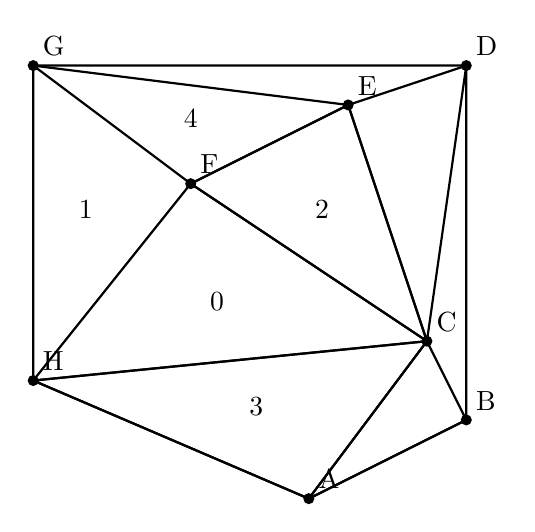
\begin{tikzpicture}
    % Define the points
    \coordinate (A) at (4,0);
    \coordinate (B) at (6,1);
    \coordinate (C) at (5.5, 2);
    \coordinate (D) at (6, 5.5);
    \coordinate (E) at (4.5, 5);
    \coordinate (F) at (2.5, 4.0);
    \coordinate (G) at (0.5, 5.5);
    \coordinate (H) at (0.5, 1.5);
    
    % Draw the points
    \foreach \point in {A,B,C,D,E,F,G,H}
      \fill (\point) circle (2pt);

    \node[above right] at (A) {A};
    \node[above right] at (B) {B};
    \node[above right] at (C) {C};
    \node[above right] at (D) {D};
    \node[above right] at (E) {E};
    \node[above right] at (F) {F};
    \node[above right] at (G) {G};
    \node[above right] at (H) {H};

    
    % Draw the convex hull
    \draw[thick] (A) -- (B) -- (D) -- (G) -- (H) -- cycle;
    
    \onslide<2->{
        \draw[thick] (A) -- (B) -- (C) -- cycle;
        \draw[thick] (A) -- (C) -- (H) -- cycle;
        \draw[thick] (H) -- (C) -- (F) -- cycle;
        \draw[thick] (C) -- (E) -- (F) -- cycle;
        \draw[thick] (C) -- (E) -- (D) -- cycle;
        \draw[thick] (E) -- (F) -- (G) -- cycle;
    }

    \onslide<3->{
        \coordinate (CenterHFC) at (barycentric cs:H=1,F=1,C=1);
        \node at (CenterHFC) {0};
        
        \coordinate (CenterHFG) at (barycentric cs:H=1,F=1,G=1);
        \node at (CenterHFG) {1};

        \coordinate (CenterCEF) at (barycentric cs:C=1,E=1,F=1);
        \node at (CenterCEF) {2};

        \coordinate (CenterACH) at (barycentric cs:A=1,C=1,H=1);
        \node at (CenterACH) {3};

        \coordinate (CenterFEG) at (barycentric cs:F=1,E=1,G=1);
        \node at (CenterFEG) {4};

    }

  \end{tikzpicture}
